\section{L7}


\subsection{CCA-security}

CCA = Chosen Ciphertext Attack

允許攻擊者使用 decryption oracle,給予其密文,它會回傳明文。但限制攻擊者不可使用欲 challenge 的密文 \(c^\ast\)。
\begin{center}
	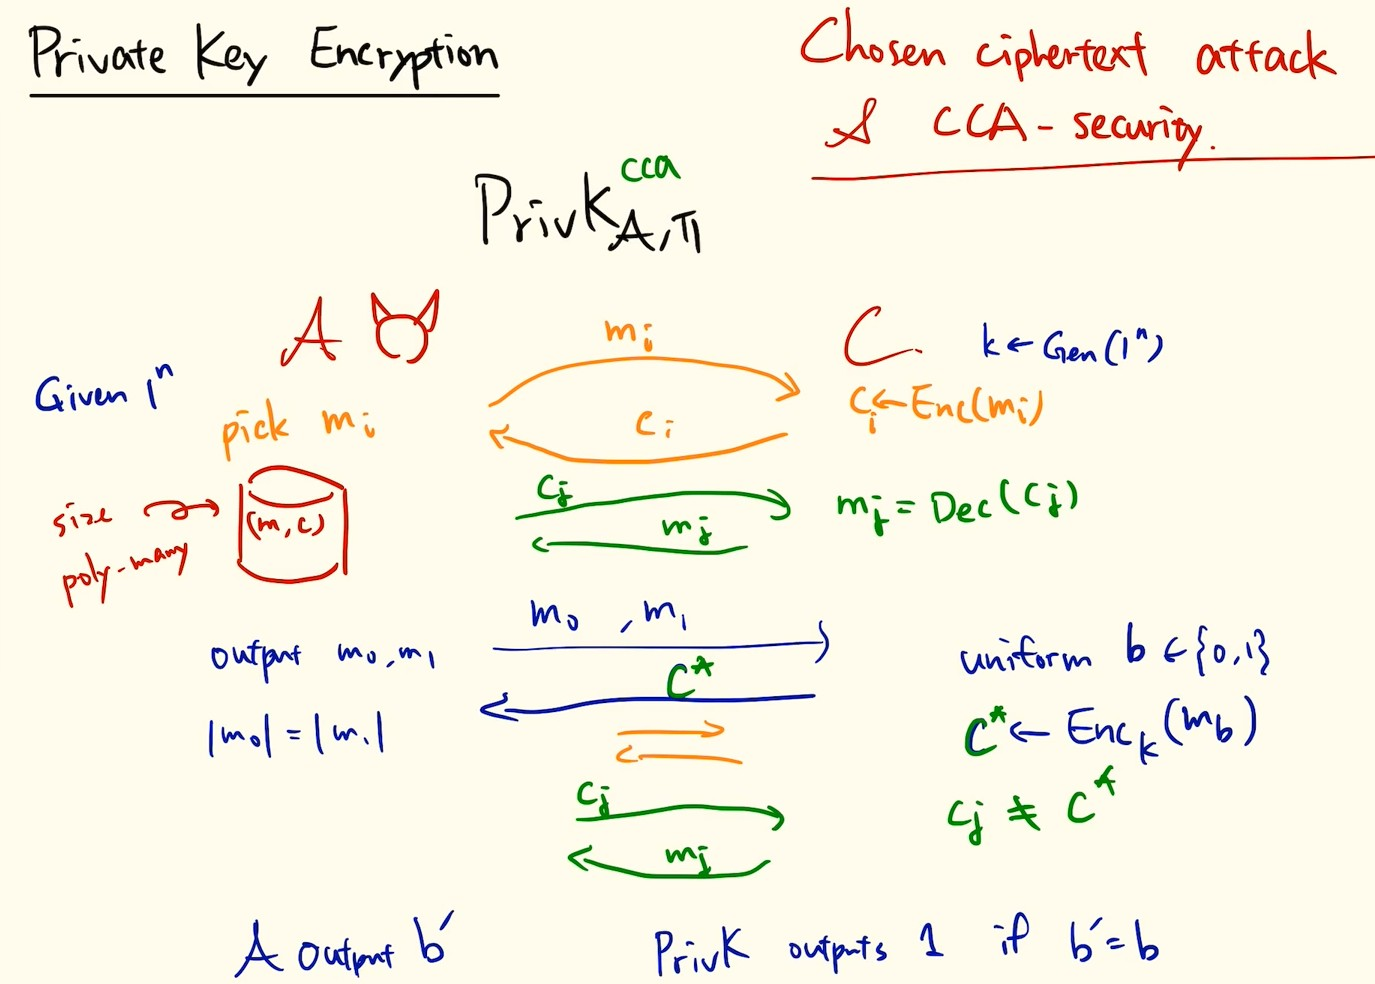
\includegraphics[width=\textwidth, keepaspectratio]{CCA_scenario.jpg}
\end{center}


\paragraph{Remark on CCA-security}

CCA => Lunch time attack

Is CCA realistic(現實可行)? \\
No, but still have weak decryption oracle which only leak 1-bit message from decrypted ciphertext, which is suffice to learn the entire message (plaintext).


\paragraph{Padding for Arbitrary Length}

Assuming block size is \(L\) bytes. \\
If message length = \(L(t-1)+2\), then we need padding which is \(L-2\) bytes.

One of the pratical padding solution is PKCS \#5:
\begin{myItemize}
	\item Block length: \(L\) byte
	\item \(b\) bytes to apppend the message to a multiple of \(L\), where \(1 \leq b \leq L\). Note that \(b \neq 0\).
	\item Append \(b\) (encoded 1 byte), b time(s). \\
	i.e., b=3 \(\Rightarrow\) 0x\underline{03} \underline{03} \underline{03}, where underlines indicate 1 byte.
\end{myItemize}

\subparagraph{Quiz}

當最後一個 block 本來就是滿的,應該如何進行 padding?

Ans: \\
額外補上一個 block,並在每個 byte 填入 block size 大小的數值。 \\
E.g. 設 block size 為 8 bytes,則額外新增一個 block,並在八個 bytes 中填入 0x08。


\paragraph{Decryption}

使用 CBC mode 解密。 

在 decryption 後檢查 encoded data,設最後一個 byte 為 \(b\):
\begin{myItemize}
	\item 若 \(b = 0\) 或 \(b > L\),return error
	\item 若最後 \(b\) 個 bytes 並不全都等於 \(b\),return error
	\item 否則,去除 padding 的部分,並 return message
\end{myItemize}


\subparagraph{Quiz}

\begin{center}
	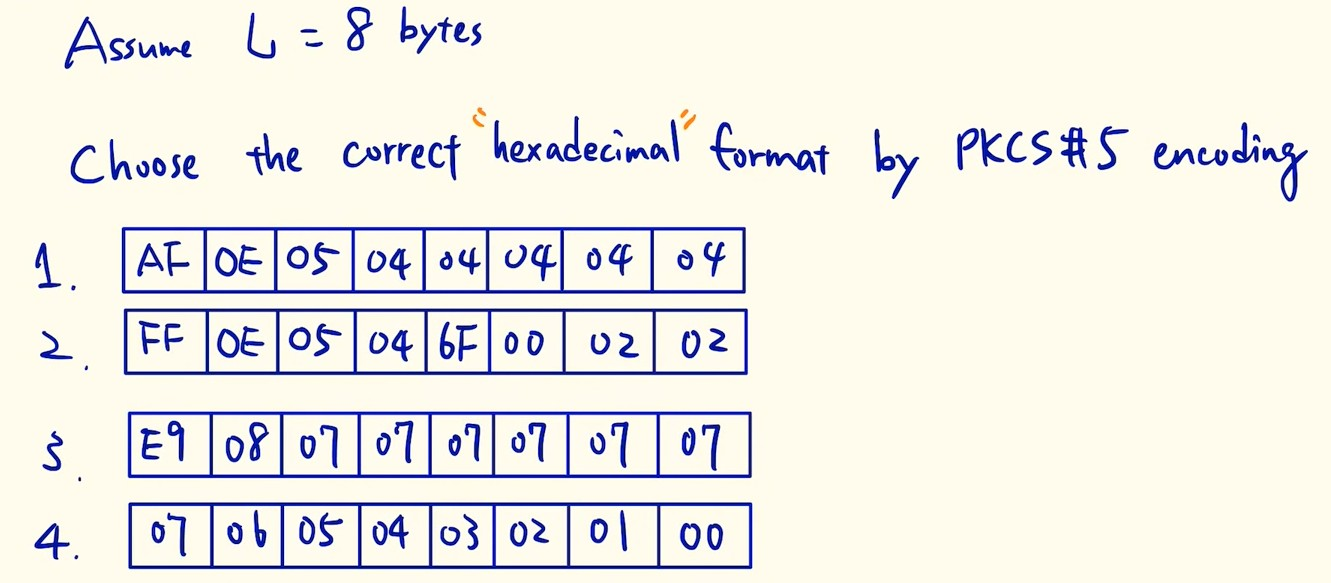
\includegraphics[width=\textwidth, keepaspectratio]{quiz_padding.jpg}
\end{center}

Ans: (2)


\paragraph{Weak CCA with Padding Oracle}

這裡出現了一種新的 oracle。給定 ciphertext,它會 return padding 是正確或錯誤。

\begin{center}
	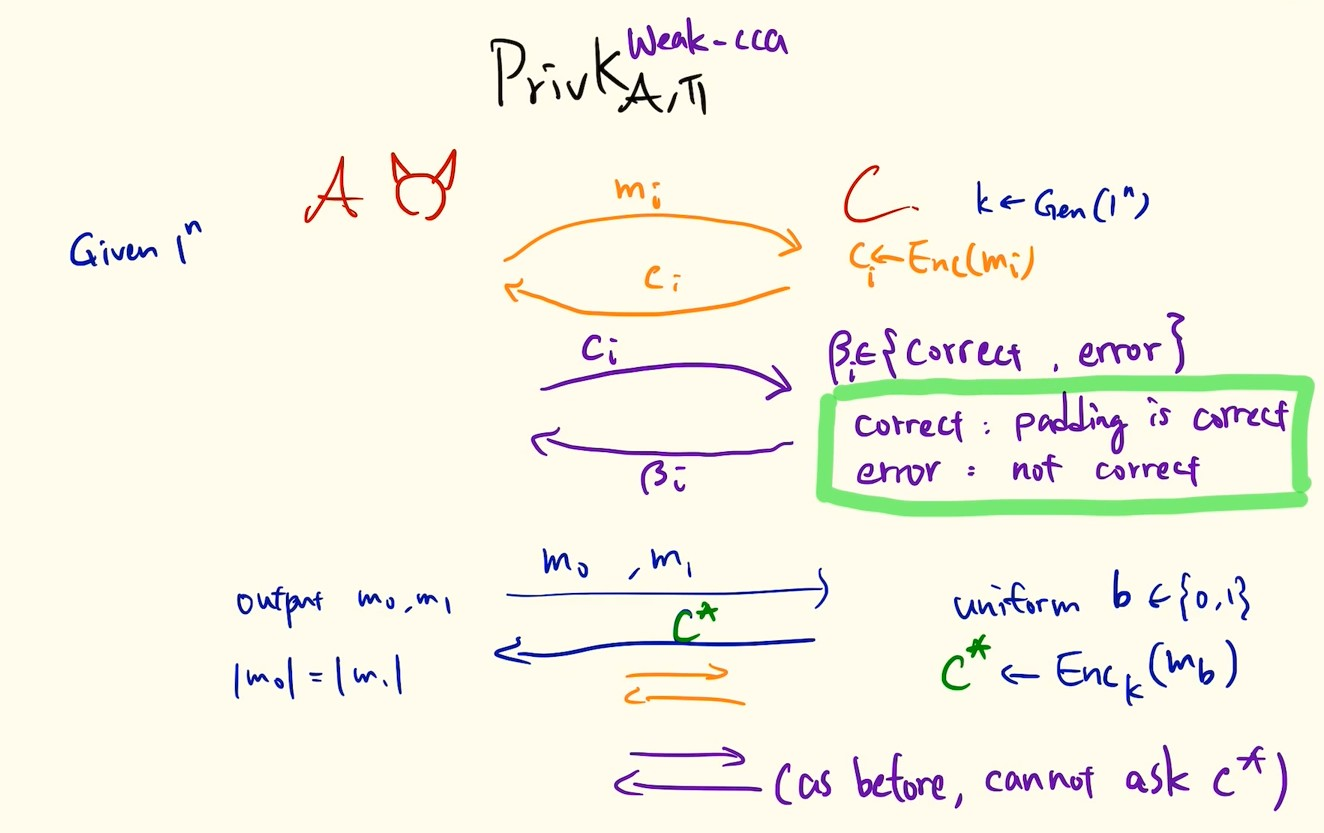
\includegraphics[width=\textwidth, keepaspectratio]{weak_cca_scenario.jpg}
\end{center}


\paragraph{Padding Oracle Attack}

\subparagraph{基本原理}

\begin{center}
	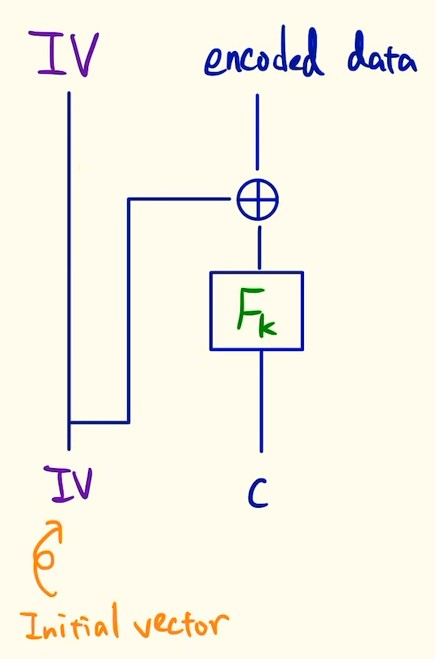
\includegraphics[width=0.2\textwidth, keepaspectratio]{padding_oracle_attack_basics.jpg}
\end{center}

其中 encoded data = \(F_k^{-1}(c) \oplus IV\)

我們可以觀察到,若 attacker \(A\) 修改了 IV 的第 \(i\) 個 byte,這個動作只會影響到 encoded data 的第 \(i\) 個 byte。(\(\because\) CBC 使用 XOR 運算)

\subparagraph{攻擊過程}

Attacker 會先由左至右逐個修改 byte,並在每次修改完之後都詢問 oracle。直到 oracle return error,該 byte 到最右邊即為 padding bytes:
\begin{center}
	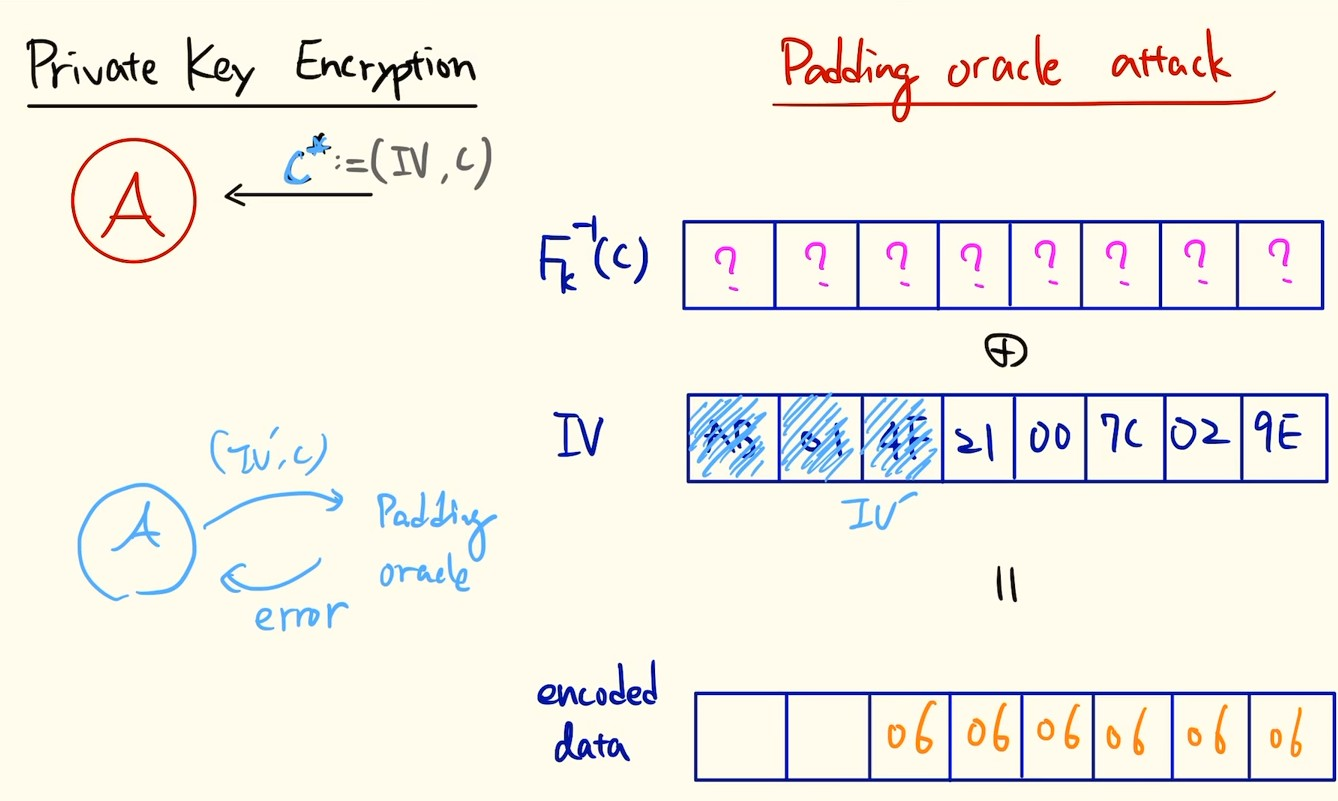
\includegraphics[width=0.8\textwidth, keepaspectratio]{padding_oracle_attack_1.jpg}
\end{center}

之後 attacker 便可藉由 IV 和 encoded data 反推 \(F_k^{-1}(c)\) 的 padding 部分為何:
\begin{center}
	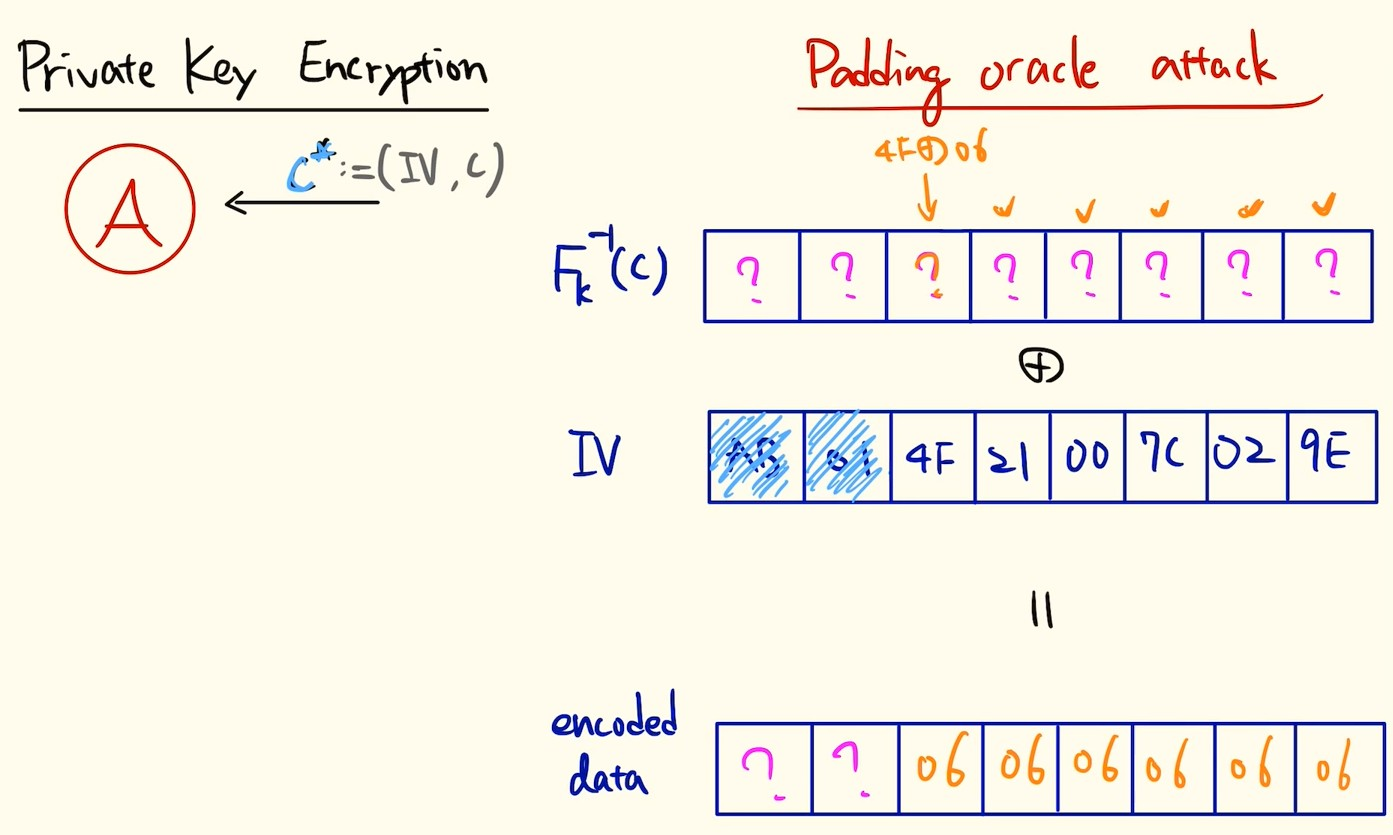
\includegraphics[width=0.8\textwidth, keepaspectratio]{padding_oracle_attack_2.jpg}
\end{center}

為了得到非 padding 部分的 message 為何,attacker 可以藉由修改 padding 部分為原本的值再加一,並重新計算新 IV 的 padding 部分:
\begin{center}
	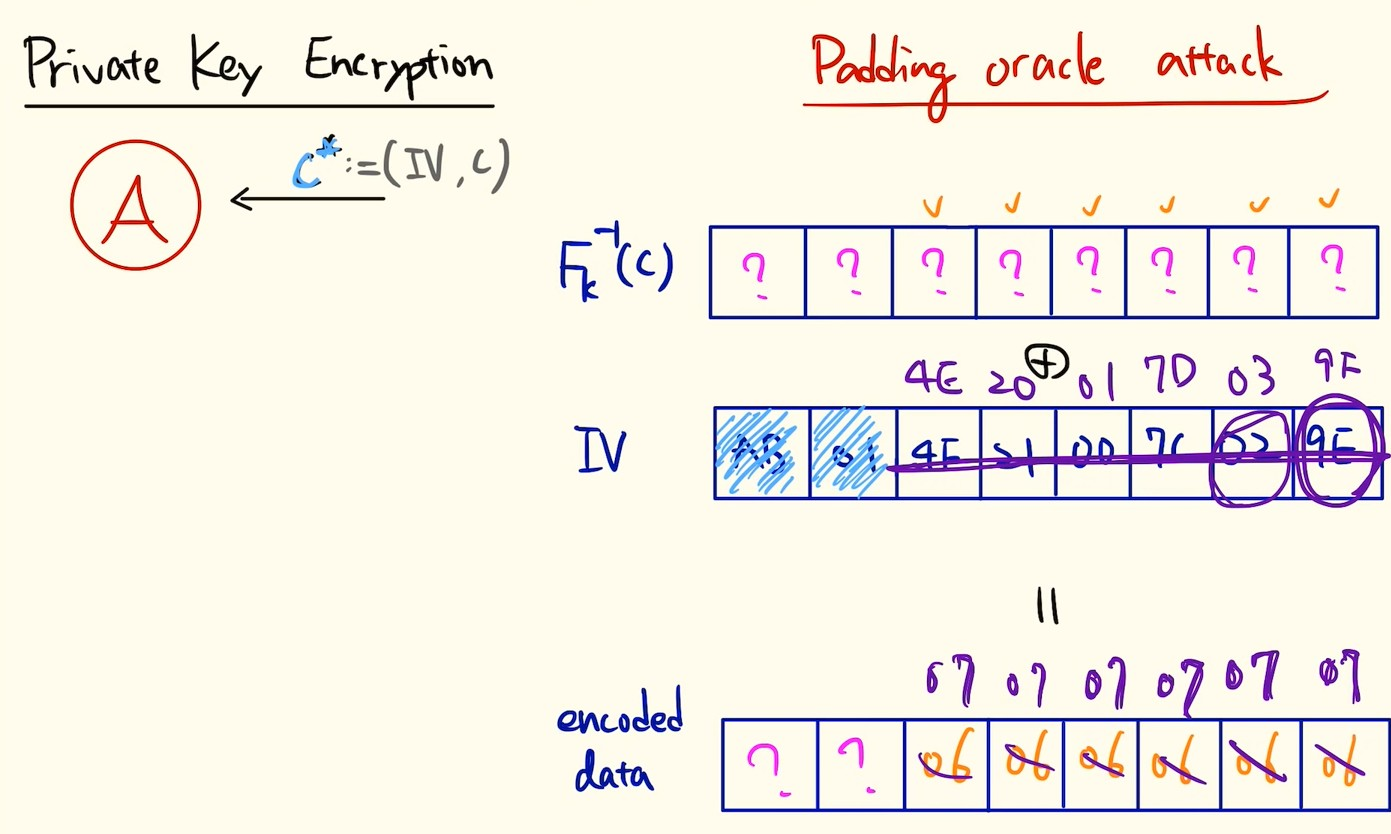
\includegraphics[width=0.8\textwidth, keepaspectratio]{padding_oracle_attack_3.jpg}
\end{center}

再來是持續修改非 padding 部分的最後(最右)一個 byte,直到 padding oracle return correct,attacker 就可以知道此時的 encoded data 中的對應 byte 為原本的 padding 值再加一。最後依序計算 \(F_k^{-1}(c)\) 得到密鑰,再將密鑰與 IV 做 XOR 得到原本的 encoded data。
\begin{center}
	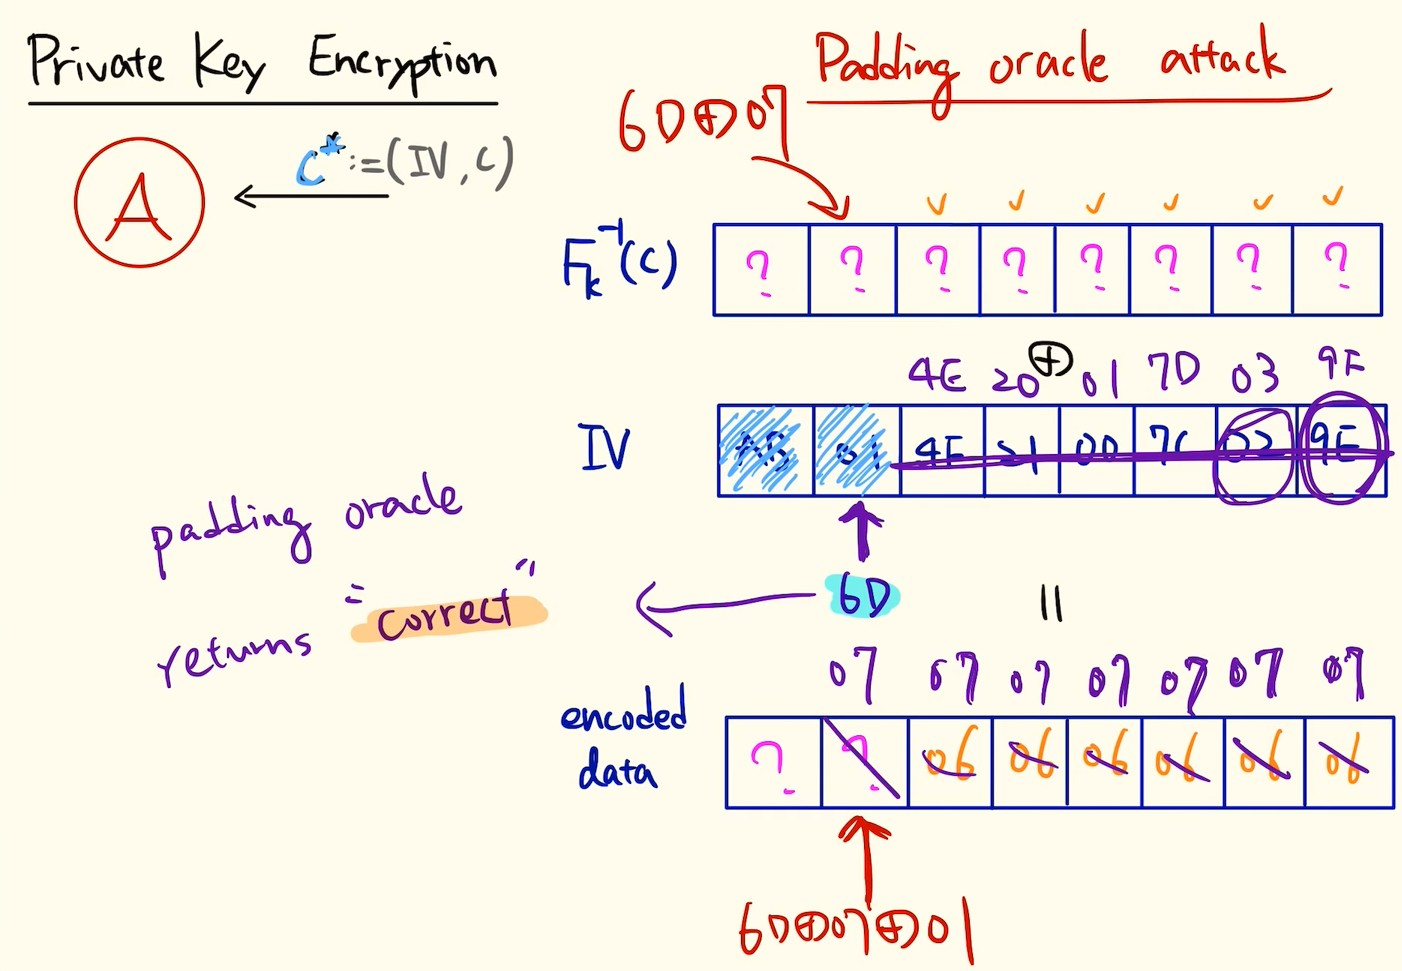
\includegraphics[width=0.8\textwidth, keepaspectratio]{padding_oracle_attack_4.jpg}
\end{center}

持續進行這些步驟就可以得到完整的 encoded data 為何。

\subparagraph{Remark on Padding Oracle Attack}

\begin{myItemize}
	\item \# of pading bytes: \(< L\) padding oracle queries(確定 padding byte 的數量所需的次數)
	\item contain of one byte of the message: \(\leq 2^8 = 256\) padding oracle queries(最多嘗試 256 次即可猜到 encoded data 中非 padding 部分的一個 byte)
	\item In \(PrivK^{weak-cca}_{A, \Pi}\) with padding oracle, \(A\) choose \(m_0, m_1\) such that \(|m_0| = |m_1|\) and last significant byte of \(m_0\)is different from correspondence of \(m_1\). And it only needs \(\leq L + 2^8\) padding oracle queries to finish it.
\end{myItemize}


\subsection{Message Authentication Code (MAC)}


Secrecy:\parbox{\linewidth}{由 \(\Enc\) 提供、adversary 無法知道訊息內容、不能涵蓋所有的 concerns(例如:訊息篡改)} \\
Integrity:確保訊息不被篡改 (tampering)、驗證訊息的正確性

MAC = Message Authentication Code


\paragraph{Syntax}

Alice 傳 message \(m\) 及一個可以驗證 message 的 tag \(t\) 給 Bob,而 Bob 在收到訊息後,透過 \(t\) 來驗證 \(m\)。

\(\Pi\) is a MAC construction.
\(\Pi = (\Gen, \Mac, \Vrfy)\)
\begin{myItemize}
	\item Key generation \(\Gen(1^n) \rightarrow k\): a key
	\item Message authentication code \(\Mac(k, m) \rightarrow t\): a tag
	\item Verification \(\Vrfy(k, m, t) \coloneq 0 \text{ or } 1\), where 0 stands for rejection, 1 stands for acceptance.
\end{myItemize}

\subparagraph{Remark}
\begin{itemize}
	\item \(m\) is not hidden for \(\Vrfy\).
	\item 對於一個 deterministic MAC,\(\Vrfy\) 在做的事情就是重新建立一次 \(t\),並比較其是否與接收到的 \(t\) 相同。
	\item If \(m \in \{0, 1\}^{l(n)}\) where \(l(n)\) is a polynomial, then MAC is fixed-length MAC.
\end{itemize}


\paragraph{Experiment \quad \(\displaystyle \MacForge_{A, \Pi}(n)\)}

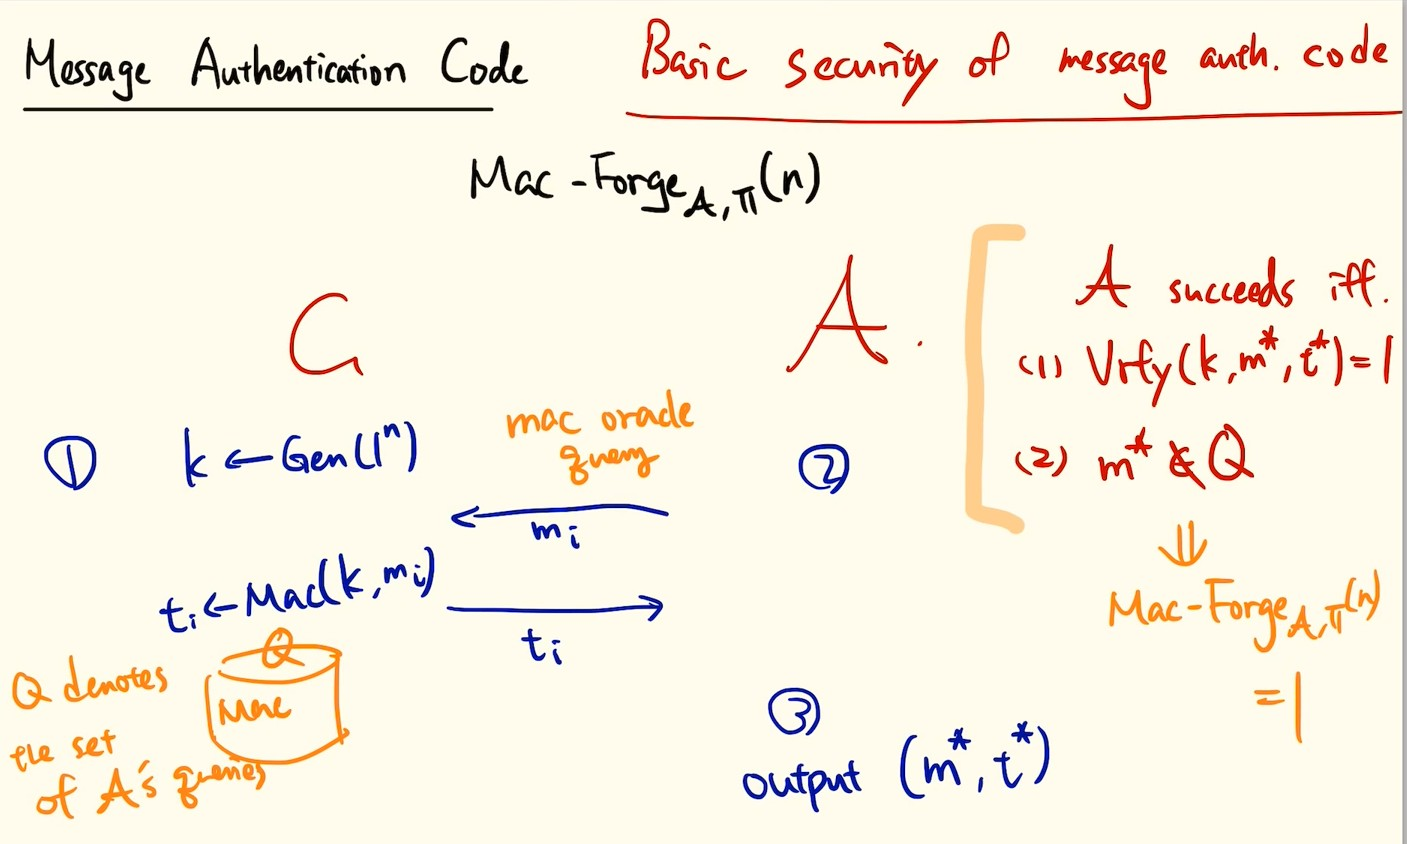
\includegraphics[width=0.8\textwidth, keepaspectratio]{MacForge_scenario.jpg}

有 challenger \(C\) 和 adversary \(A\):
\begin{steps}
	\item \(C\) 產生 key,即 \(k \leftarrow \Gen(1^n)\)
	\item \(A\) 選擇一個 message \(m_i\),以此詢問 \(C\),而 \(C\) 再 return 一個計算過後的 tag \(t_i \leftarrow \Mac(k, m_i)\) 給 \(A\)。此外,\(C\) 可以使用一個 list \(Q\) 來收集所有來自 \(A\) 的 queries。
	\item \(A\) outputs 他的偽造 \((m^\ast, t^\ast)\)
\end{steps}

\(A\) 成功的條件(即 \(\MacForge_{A, \Pi}(n) = 1\))有兩個(都要符合,if and only if):
\begin{enumerate}[topsep=-\parskip, label=(\arabic*)]
	\item \(\Vrfy(k, m^\ast, t^\ast) = 1\)
	\item \(m^\ast \not\in Q\)
\end{enumerate}

\subparagraph{Remark}

\(\MacForge\) 的 strong 版本是\(\MacSForge\)。 \\
\(\MacSForge\):比 \(\MacForge\) 寬鬆一點,只要求 \((m^\ast, t^\ast)\) 也不在 \(Q\) 中,即 \((m^\ast, t^\ast) \not\in Q\)。

If a deterministic MAC satisfies existential unforgeability in \(\MacForge\), it also satisifeis strong unforgeability in \(\MacSForge\). \\
解釋:因為 deterministic MAC 會將一個 \(m\) 只對應到一個 \(t\),所以如果 \(m^\ast\) 不在 \(Q\) 中,則與之對應的 \(t^\ast\) 也不會在 \(Q\) 中。因此 \((m^\ast, t^\ast) \not\in Q\)。


\paragraph{Strong Verison of Previous Experiment \quad \(\MacSForge_{A, \Pi}(n)\)}

大致和之前相同,唯一不同處在於 \(A\) 成功的第二個條件改成 \((m^\ast, t^\ast) \not\in Q\)。這意味著 \(A\) 可以向 \(C\) query \(m^\ast\),但只要可以偽造另一組不在 \(Q\) 中的 \((m^\ast, t^\ast)\) 並且仍可以使用它通過 \(\Vrfy\),那麼就算 \(A\) 成功了。

只要在 \(\MacSForge\) 是安全的,那它在 \(\MacForge\) 也是安全的。反之則不成立。
\begin{definition}[Strong Security]
	\[ \Pr[\MacSForge_{A, \Pi}(n) = 1] \leq \negl(n) \]
\end{definition}


\paragraph{Security Definition of MAC}

\begin{definition}
	A message authentication code \(\Pi = (\Gen, \Enc, \Vrfy)\) is existentially unforgeable under adaptive chosen message attacks, if for all PPT adversaries \(A\) there is a ngeligible function \(\negl\) such that
	\[ \Pr[\MacForge_{A, \Pi}(n) = 1] \leq \negl(n) \]
\end{definition}


\paragraph{Construction}

\subparagraph{Pseudorandom Function}

Pseudorandom function (PRF) 的定義請參見 \fullref{PRF}。

\subparagraph{Construction of Fixed-length MAC}

Let \(F: \{0, 1\}^n \times \{0, 1\}^n \rightarrow \{0, 1\}^n\) be a PRF. \\
\(\Pi = (\Gen, \Mac, \Vrfy)\) is a fixed-length MAC for message fo length n.
\begin{myItemize}
	\item \(\Gen(1^n)\): uniform \(k \in \{0, 1\}^n\)
	\item \(\Mac(k, m)\): on input \(k\) and message \(m \in \{0, 1\}^n\), outputs a tag \(t = F_k(m)\) where \(t\) is \(t\)-bit tag.
	\item \(\Vrfy(k, m, t)\): on input \((k, m, t)\), outputs 1 if and only if \(t = F_k(m)\); otherwise, outputs 0.
\end{myItemize}
